\chapter{Introduction}
\label{chap:introduction}


% Intro usually also is an expanded higher-level summary of the thesis contributions and the overall theme.
% Right place to emphasize the key underlying conceptual contributions [locality, performance, control-plane scaling and simplicity]
% Try thinking of a figure/table to put all chapters/contributions in context. 
% Will also help for the slides. 
% So things like keep-alive, load-balancing, control-plane, etc. 
% You had something in the proposal slides similar to this? Shows the layers and components and illustrates you have comprehensively addressed the problem.

% This thesis examines the current state of serverless computing control planes from both a provider, researcher, and user perspective, and proposes improvements to all these facets.
This thesis describes the current state of a new computing paradigm, \emph{serverless computing}, and proposes improvements to various aspects of the control planes that orchestrate serverless computing systems.
Serverless computing, otherwise known as Function as a Service (FaaS) has the possibility to revolutionize cloud computing.
% It evolved out of the want to abstract away hardware from users, and increase the ability of cloud providers to manage resource utilization.
It evolved from out of the ethos of cloud computing where hardware is abstracted and \emph{rented} to customers.
% Serverless platforms totally manage users' applications using a FaaS \emph{control plane}, orchestrating deployment, execution, scaling, resources, and more.
Serverless computing is the epitome of this abstraction, where the cloud provider totally manages users' applications using a FaaS \emph{control plane}, orchestrating deployment, execution, scaling, resources, and more.

Traditionally, an application would be hosted by the developer using hardware that they personally owned and managed.
This causes problems when trying to rapidly scale up the number of users for the application -- additional hardware must be purchased (slowly), or the system must be over-provisioned to handle peak user load.
% Traditional cloud computing relies on rented virtual machines that end users have full control over.
Cloud computing platforms can provision new \quotes{hardware}, in the form of a \emph{virtual machine} (VM)~\cite{xen}, in a matter of minutes.
The developer then deploys their application onto the VM and can connect it to the existing cluster of machines.
When user load decreases, say at night, these VMs can be deleted and do not have to be paid for.
% Not just control, but responsibility for deploying and scaling their application, managing and patching an OS, and paying the cost even when the application is not being used.
% Users want to skip these hassles, minimize costs, and focus on developing their applications.

At the same time, software development practices were pushing to split up large monolithic applications into functionality-specific \emph{microservices}.
Deploying microservices onto individual VMs lead to wasted resources and high orchestration overhead.
Developers started to ship their applications inside pre-packaged \emph{containers}~\cite{docker-main}, that contained all necessary dependencies for it to run.
Platforms~\cite{kubernetes} were also created that could deploy these containers and manage the services within them using some simple configuration.
Cloud providers could then run these orchestration tools on their hardware, and deploy user-provided containers directly.

This approach is highly popular today, but has several drawbacks and overheads.
Containers reduce, but do not wholly eliminate duplicate state, often consisting of several hundred MBs of dependencies.
Developers still need to be aware of when, where, and how their application would run, now more convoluted because \emph{they} were responsible for putting this together themselves.
Mitigating such problems and reducing developer overhead required specialist \quotes{DevOps} positions to handle the complexity of deploying software. 
% Idle services could be eliminated, but only if configured in certain ways.
Idle services can not be eliminated at the granularity of container orchestration, so possible minutes of idle time between serving requests must be paid for.


Serverless computing completes this transition by taking responsibility for all of these concerns.
Individual serverless \emph{functions} are typically small, which are created by developers by directly uploading source code to the provider.
It is then responsible for preparing the function's dependencies, and executing it when a request with arguments comes in.
The user is only billed for resources used \emph{during} this execution time, a unique shift in billing costs.
Several functions can be chained into a complex \emph{application} via a directed acyclic graph (DAG) description.
The low-maintenance and pay-per-use model has proven highly attractive to customers, and FaaS growth since its inception in 2014~\cite{lambda} has been dramatic.
% Cloud customers want to easily deploy and scale their applications at a minimum cost and effort to themselves.
% Serverless computing has become a forerunner in meeting both of these demands.
% Its pay-per-use pricing model and guarantee by the provider to scale up compute instances with demand alleviate complexity for end users.
% Since its introduction in 2014~\cite{lambda} it has grown in orders of magnitude in number of invocations served, viable use cases, and research popularity.

% At the same time, cloud providers are constantly seeking for new ways of monetizing unused compute resources and maximizing control over their resources.
% FaaS has emerged as a successful way of achieving both of these ends.
Cloud providers are pushing users to this new platform because they get several benefits from this style of computing.
%  monetizing unused compute resources and maximizing control over their resources.
% The small and ephemeral nature of functions allows for fine-grained control by the provider along a number of axes. 
A function's resources are considered \emph{ephemeral}, and can be removed at the provider's discretion when not being used.
The resource demands of a function are much smaller than that of a VM or container, allowing many hundreds to be hosted on a single \emph{worker}.
Many invocations can be run on a worker at a time, and the provider can load-balance these to maximize utilization of their clusters that are plagued by wasted resources~\cite{fuerst2020cloud,fuerst2022memory,wang2021smartharvest,serverless-harvest-sosp21,harvest-osdi20}.
The transition to more fine-grained resource management allows for more advanced optimizations and opportunities for improving resource utilization.

Achieving this detailed level of control such features comes with an equal complexity cost for the control plane that is to orchestrate it.
The value in serverless comes from its ability offer low-latency \emph{performance}, which requires a \emph{simple yet scalable} control plane providing \emph{locality}.
The primary components of such a control plane are outlined in Figure~\ref{fig:control-plane}, citing where this thesis has impacted.
A worker executing serverless functions can host dozens of concurrent executions and thousands of idle functions to fully utilize resources (Chs.~\ref{chap:faascache}\&\ref{chap:gpu-sched}).
The entire control plane coordinates the execution of billions of invocations per day~\cite{sahraei2023xfaas} and must scale to clusters of thousands of machines, guaranteeing good performance under uncertain conditions (Chs.~\ref{chap:chrlu}\&\ref{chap:iluvatar}).
Active work on serverless spans from low-level virtualization and OS abstractions to high-level scheduling and load-balancing (Ch.~\ref{chap:chrlu}) algorithms.
This thesis discusses issues existing in current FaaS control planes and proposes methods, new designs, and future-thinking systems to tackle them.

\begin{figure}
  \centering
  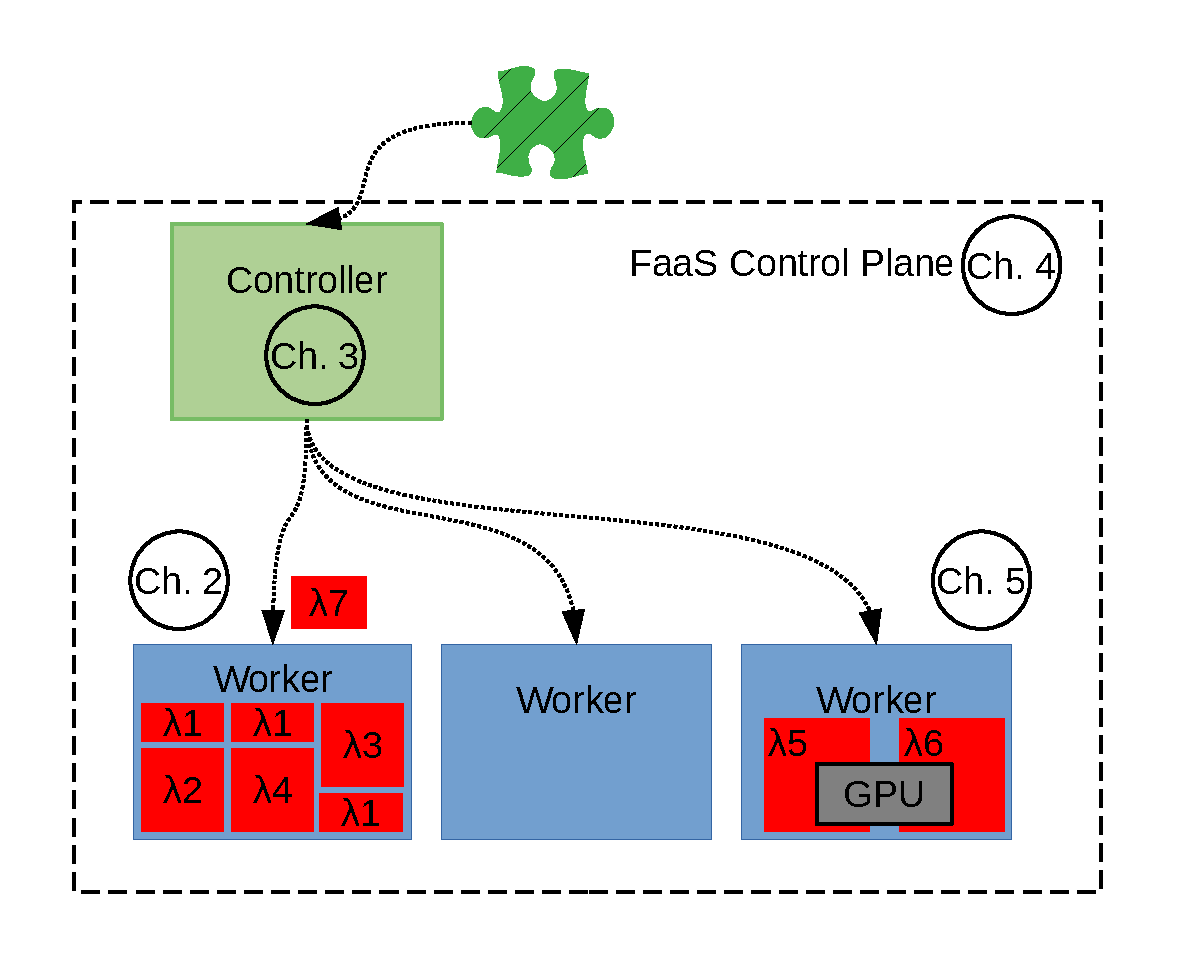
\includegraphics[width=\textwidth]{introduction/figs/faas-labeled.pdf}
  \caption{The major components of the control plane, and the areas of each this thesis impacts.}
  \label{fig:control-plane}
\end{figure}

FaaS control planes themselves have been designed, re-design, and ported to a variety of ecosystems to solve unique problems and constraints.
% Nor is it a single "design" or platform
FaaS has been placed along the edge-to-cloud continuum~\cite{cicconetti2020decentralized,russo2023serverless,cheng2019fog,wang2020supporting}, taking advantage of its scale-to-zero capability.
% heterogeneous hardware
Moving serverless platforms beyond cloud computing to heterogeneous hardware has been explored~\cite{du2022serverless}, which is key for integration of IoT~\cite{persson2017kappa,trilles2020iot,cheng2019fog,wang2020supporting} and FPGA~\cite{bacis2020blastfunction,ringlein2021case} hardware.
% Private (Meta) 
Meta created an internal FaaS platform~\cite{sahraei2023xfaas} which could be optimized using their knowledge of what workloads run on it.
% FuncX
Another unique entry, FuncX~\cite{funcx_hpdc_20}, creates a layer over supercomputing resources to run user experiments in a FaaS-like manner.
% Cloud - GCP, Alibaba, AWS, Azure, several others
The most well-known platforms are the public offerings of the major cloud providers, AWS Lambda~\cite{lambda}, Google Functions~\cite{gcp-functions}, Azure Functions~\cite{azure-functions}, and Alibaba Function Compute~\cite{alibaba-compute}.
Several open-source equivalents have been made~\cite{openwhisk,openfaas,nuclio,knative} which are popular in both research and as products for end-users.
Included in this thesis is a design for a fitter-free, low-latency control plane and is highly configurable and able to run on heterogeneous and edge hardware.

% FaaS research isn't limited to a single domain
More focused research into serverless has branched into nearly every field of systems research.
To serve a function invocation, the system must create an isolated \emph{sandbox} to execute the user code in.
% A variety of isolation techniques predate FaaS~\cite{docker-main}, and were
Numerous isolation mechanisms have been put forward, containers~\cite{chhatrapati2021towards,docker-main,gvisor}, language runtimes~\cite{shillaker2020faasm,aytekin2019harnessing}, and lightweight virtualization~\cite{firecracker-nsdi20}.
All of these take time to start, in what's referred to as a \textit{cold starts} and can significantly increase invocation latency.
Additional research has targeted this problem specifically to accelerate existing isolation mechanisms creation time~\cite{mohan2019agile,du2020catalyzer,warm2}.
Future invocations see lower latency by benefiting from \emph{locality}, re-using the isolation sandbox in a \textit{warm start} invocation.

Knowingly keeping idle sandboxes resident in memory improves latency, but may lead to resource underutilization.
Sandboxes sizes are chosen by users, who often over-provision to negate performance problems~\cite{mvondo2021ofc,romero2021faa,eismann2021sizeless,yu2021harvesting,serverless-harvest-sosp21}.
Worker nodes also cannot host a container per function, who often require several for ideal performance, therefore remove them periodically to conserve space~\cite{faascache-asplos21}.
The highly heterogeneous workload of FaaS has proven challenging when trying to predict when containers will be needed, which would allow their removal from memory to conserve resources~\cite{shahrad2020serverless,zhao2021understanding}.
Adjusting the number of containers a function has reduces footprint, but may impact latency as they cannot be shared~\cite{enes2020real,li2022kneescale}.
Maintaining locality to provide acceptable performance while maximizing use of resources is an open area of research and addressed here.
% Keeping isolation containers around to serve future invocations requires their state to be maintained, typically in-memory.
% All possibly containers cannot be kept around because server resources are limited and valuable.
% The \textit{keep-alive} decision selects if and/or when containers are removed.


FaaS by design exists at a cluster level, so we cannot consider its challenges solely from a single-worker perspective.
Functions have a variety of characteristics: execution time, inter-arrival-time of invocations, memory usage, and more.
These can all vary in orders of magnitude, from 0.1 s - 60 s runtimes to sub-second to daily invocation arrivals~\cite{shahrad2020serverless}.
% The control plane is expected to guarantee low latency in all cases and scale applications up or down with changing demand.
Even worse, functions are notoriously bursty, rapidly changing how frequently invocations occur.
% In all, a FaaS control plane must handle millions of invocations per day and run them on clusters of thousands of machines.
% One could schedule function sandboxes, distinct from load balancing invocations~\cite{balaji2021fireplace,kaffes2021practical,abdi2023palette}, is a related problem to evenly distribute work across the cluster as functions vary with how many invocations they have.
One could schedule function sandboxes~\cite{balaji2021fireplace,kaffes2021practical,abdi2023palette,openwhisk} and have the controller micro-manage the cluster state.
% We must load balance~\cite{aumala2019beyond,leegreedy} invocations across clusters of servers and avoid overload any individual.
Load balancing invocations~\cite{aumala2019beyond,leegreedy,faaslb-hpdc22} is a more scalable way to address the complex load and large cluster uncertainty, trusting workers to make ideal decisions.
The cluster control plane targets locality in both cases, knowing that running invocations in existing sandboxes is much more performant.

Cloud providers currently do not expose compute capabilities outside of CPU computation, but users want to put latency-critical applications like ML inference onto FaaS platforms to take advantage its high scalability.
% Serverless functions currently cannot viably access CPU parallelism, and are configurable to use a limited number of CPU cores during execution. 
Accelerators come in many flavors: SmartNICs~\cite{choi2020lambda}, GPUs~\cite{pemberton2022kernel,guleria2019emf}, FPGAs~\cite{bacis2020blastfunction}, and more~\cite{du2022serverless,romero2021llama} -- each with unique characteristics and types of applications they can support.
A host of applications are lining up~\cite{yang2022infless,ali2022optimizing,zhang2019video,risco2021gpu,hung2019rapid,shankar2020serverless} to run on faster FaaS hardware.
FaaS invocations are also unable to easily coordinate computation with each other~\cite{yuan2022smpi,copik2023fmi,copik2022faaskeeper,sreekanti2020fault,sreekanti2020cloudburst,giantsidi2023flexlog,xu2021lambdadnn}, requiring slow intermediaries for interaction.
These accelerators also require locality to achieve usable performance, having significant and often longer cold start times.
% They also have a secondary effect
A unique \emph{data locality} for these devices exists too, as they must have data on hand that may have been cached on a system with more available memory.
Running accelerated and massively parallel computation in FaaS that puts not restrictions on applications is important for adoption and continued growth.

% security~\cite{kim2023cryonics,zhao2023reusable,trach2019clemmys}
% applications~\cite{zhang2021serverless,mete2021implementation,hussain2019serverless,fouladi2019laptop,copik2022faaskeeper,hung2019rapid}
% % edge
% Edge serverless computing~\cite{aslanpour2021serverless,raith2023serverless,russo2023serverless}

% Domain-specific targets
% Low-latency~\cite{jia2021nightcore}
% Lang Runtime~\cite{shillaker2020faasm}
% FaaS as collection of services
% BaaS~\cite{baas,giantsidi2023flexlog,sreekanti2020cloudburst,sreekanti2020fault}


% Allows various trade-offs, in performance, security, and features.
% Serverless control planes have significantly different challenges and research opportunities than VM-based cloud computing.

\section{Thesis Outline}

This thesis is consists of five additional chapters and is ordered as follows.
The following chapter~\ref{chap:serverless} provides in detail what serverless computing is, what technologies it builds on top of, and how it is being used in both research and by users.
Serverless evolved from, and is still built on top of, abstractions in cloud computing like virtual machines (VMs) and containers.
These mechanisms are used to isolate functions from one another and allow the control plane to control and protect resources.
This control plane itself consists of several components, a \emph{controller}, \emph{workers}, and ancillary services.
Users interact with the controller to create functions, invoke them, and receive results.
It, in turn, load balances invocations amongst the cluster of workers that execute them using the aforementioned isolation tools.
The many and varied designs presented by researches are shown and compared here.
Techniques to improve isolation mechanism performance and load balancing are frequent.
Wholly new systems have also been built, typically targeting a specific workload class such as machine learning (ML), which has become popular in serverless.
This exploration ends with a detailing of the many use cases serverless has been put towards, including ML, scientific computing, and even distributed computing.

Chapter~\ref{chap:faascache} has the first contribution of this thesis and describes a container cache management design called \emph{FaasCache}.
%, and is about making smarter decisions in when to remove function containers.
Control planes keep idle function containers resident in memory in the expectation that they will be used again in the future.
These warm executions are significantly faster than their counterparts that must wait for a container to be spun up.
% In order to achieve low latency for individual function invocations, FaaS control planes must keep execution sandboxes resident in memory.
Unfortunately, memory is neither a free nor infinite resource, so control planes remove containers to both conserve and make room for others.
FaasCache optimizes worker memory usage by treating these containers as a \emph{cache}, and carefully considers what to evict when under resource constraint.
Each worker monitors function characteristics such as memory usage, frequency, and container startup time.
These are fed into a policy deciding which will be more valuable to keep given the cost of having to re-create it and how soon that might be.
It also monitors the cache-hit ratio of invocations to dynamically resize the memory allocated to the cache for targeting performance.
% This eviction decision is usually done on a timeout started when the last time a container was used.
% In this work I propose switching to on-demand resource reclamation and use several function and container attributes to decide what to remove.
% This algorithm applies ideas from the long-studied area of caching algorithms, who maximize utility out of fixed size resource pools.
% Container removal is analogous to cache eviction, and an invocation with or without an existing container can be considered a cache hit or miss.


The next chapter, chapter~\ref{chap:chrlu}, moves up a level in the control plane to present a novel load-balancing algorithm. % called 
As FaasCache shows, functions benefit from running in warm containers, which is referred to as function \emph{locality}.
The heterogeneous nature of functions would imbalance workers if we sent each function's invocations to a single worker.
Some would be overloaded and suffer significant performance degradation, others sitting idle.
Our CH-RLU algorithm targets locality for functions while at the same time avoiding worker overload.
We use \emph{consistent hashing}~\cite{karger1997consistent} to give perfect locality and distribute functions amongst workers.
To detect overloads, we keep usage reports from each worker and add anticipated load from dispatched invocations to such reports.
Extremely popular functions, those with the highest frequency of invocations, also model Gaussian noise of the load impact before sending an invocation, to model overloading scenarios.
In all cases, if we predict a worker has too much work, we direct invocations away from it in a fixed pattern, maintaining locality while minimizing overloaded workers.
The effectiveness of this at both minimizing platform overhead and keeping load even across worker clusters is described at the end of the chapter.
% Serverless control planes do not operate on a single node, so load balancing algorithms are required to distribute invocations amongst workers.
% The load balancer must make a quick decision, and take into account the highly variable characteristics of functions it serves.
% A poor decision can drastically increase latency, as many functions execute in only a few milliseconds and scheduling delays can quickly exceed this.
% An algorithm must favor locality to achieve warm hits for functions, while ensuring workers are not overloaded from function frequency imbalance.
% To find this balance I propose a mixture of a function pinning load-balancing algorithm that is informed by existing load status to avoid overcommitment.
% This will minimize latency from CPU timesharing and favor warm invocation executions.

Next, Chapter~\ref{chap:iluvatar} details a new serverless control plane design called \sysname.
% created to fix problems with existing open-source offerings.
% Current open-source FaaS control planes \cite{openwhisk} are deficient in key areas for promoting scalable research in the area.
This new control plane is written in Rust and seeks to solve the deficiencies in current open-source control planes used for research~\cite{openwhisk}.
Its worker is designed to be highly modular, allowing swap-able implementations to support heterogeneous platforms and ease comparisons for research.
It supports a novel queue mechanism to support new designs that may not run all workloads immediately, or handle cases of severe resource demand/
The controller is built on a stateless design and uses the load balancing algorithm from Chapter~\ref{chap:chrlu}, relying on the worker's local knowledge for scheduling.
The third runtime component is a time-series database~\cite{influx} used to aggregate function and worker metrics, reducing communication overhead between platform components.
Finally, and a first for such systems, it has a built-in load generation suite that integrates seamlessly with both worker and load balancer.
With this, one tool can test any level of the control plane under various load conditions, and record highly detailed information for post-experimental analysis.
We use this tool to compare with other control plans and show the performance benefits of \sysname.
% They can have a variety of issues, such as significant performance spikes, a brittle code structure for modification, lock-in to various technologies, and poor setup for consistent experimentation.
% I detail a new serverless control plane that will be designed with two goals in mind: be effective for enabling research and low variability latency.
% Having a low and controlled latency is critical for having confidence in experimental results, the ability to attribute data to changes you made.
% The control plane being easily extensible and integrating seamlessly with a load generation framework is vital to productive research.

% Chapter~\ref{chap:new-poly} polymorphic functions are proposed as extensions to serverless capabilities.
% Chapter~\ref{chap:new-mpi} serverless MPI is proposed as extensions to serverless capabilities.
The final piece of this thesis is Chapter~\ref{chap:gpu-sched}, which uses \sysname~to multiplex GPU resources to serve black-box functions.
To prevent maintain control of GPU resources, we insert a \emph{shim} in between the function and GPU driver to intercept calls.
This lets us both over-subscribe memory and control when the memory is on-device or moved to the host.
We leverage the increase in memory control to allow many containers to share one GPU, creating a \emph{warm-pool} similar to that of regular CPU serverless.
As GPUs cannot support the same concurrency as many-cored CPUs, we use the queue mechanism of \sysname~to dynamically control ordering and dispatching of invocations.
The queue monitors GPU utilization and sends invocation when compute is available, moving memory around to ensure we don't overload the device.
Invocations also benefit from locality here, successive runs and having their memory available gives better execution performance.
We balance these needs with fairness, using the queue to prevent any function from starving others of device time.
The effectiveness of all these are demonstrated with thorough experimental analysis at the end of this chapter.
% Users want to run workloads, especially ML inference jobs, with low latency and this requires using accelerators.
% Modern serverless systems only expose CPU compute capabilities, while some bespoke research systems target inference-only workloads.

% Chapter~\ref{chap:summary} concludes this thesis.
